\documentclass[xetex,mathserif,serif]{beamer}
\usepackage{polyglossia}
\setdefaultlanguage[babelshorthands=true]{russian}
\usepackage{minted}
\usepackage{tabu}

\useoutertheme{infolines}

\usepackage{fontspec}
\setmainfont{FreeSans}
\newfontfamily{\russianfonttt}{FreeSans}

\definecolor{links}{HTML}{2A1B81}
\hypersetup{colorlinks,linkcolor=,urlcolor=links}

\tabulinesep=0.7mm

\newcommand{\attribution}[1] {
    \vspace{-5mm}\begin{flushright}\begin{scriptsize}\textcolor{gray}{\textcopyright\, #1}\end{scriptsize}\end{flushright}
}

\title{Практика 3: Проектирование Roguelike}
\author[Юрий Литвинов]{Юрий Литвинов\\\small{\textcolor{gray}{y.litvinov@spbu.ru}}}

\date{14.04.2022}

\begin{document}
    \maketitle

    \begin{frame}
        \frametitle{Roguelike}
        \begin{itemize}
            \item Жанр компьютерных игр, назван в честь игры Rogue, 1980 года выхода
            \item Характеризуется:
            \begin{itemize}
                \item Простой тайловой или консольной графикой
                \item Активным использованием случайной генерации
                \item Перманентной смертью персонажа и невозможностью загрузить предыдущее сохранение
                \item Чрезвычайно развитым набором игровых правил
                \item Высокой свободой действий персонажа (``игры-песочницы'')
            \end{itemize}
            \item Примеры:
            \begin{itemize}
                \item \url{https://en.wikipedia.org/wiki/NetHack}
                \item \url{https://en.wikipedia.org/wiki/Angband_(video_game)}
                \item \url{https://en.wikipedia.org/wiki/Ancient_Domains_of_Mystery}
            \end{itemize}
        \end{itemize}
    \end{frame}

    \begin{frame}
        \frametitle{Что хочется}
        \begin{itemize}
            \item Персонаж игрока, способный перемещаться по карте, управляемый с клавиатуры
            \begin{itemize}
                \item Карта обычно генерируется, но для некоторых уровней грузится из файла
                \item Характеристики --- здоровье, сила атаки и т.д.
                \item Экспа и уровни персонажа, с ростом уровня повышаются характеристики
            \end{itemize}
            \item Инвентарь персонажа, включающий элементы, влияющие на его характеристики, которые можно надеть и снять
            \item Несколько разных видов мобов, способных перемещаться по карте
            \item Боевая система --- движущиеся объекты, пытающиеся занять одну клетку карты, атакуют друг друга
            \item Все детали --- на ваше усмотрение
        \end{itemize}
    \end{frame}

    \begin{frame}
        \frametitle{Задача}
        \begin{columns}
            \begin{column}{0.5\textwidth}
                По принципам DDD разработать архитектуру Roguelike RPG

                \begin{itemize}
                    \item В командах по 3 человека
                    \item Требуется диаграмма компонентов и диаграмма (диаграммы) классов
                    \item Это может быть одна диаграмма
                \end{itemize}
            \end{column}
            \begin{column}{0.5\textwidth}
                \begin{center}
                    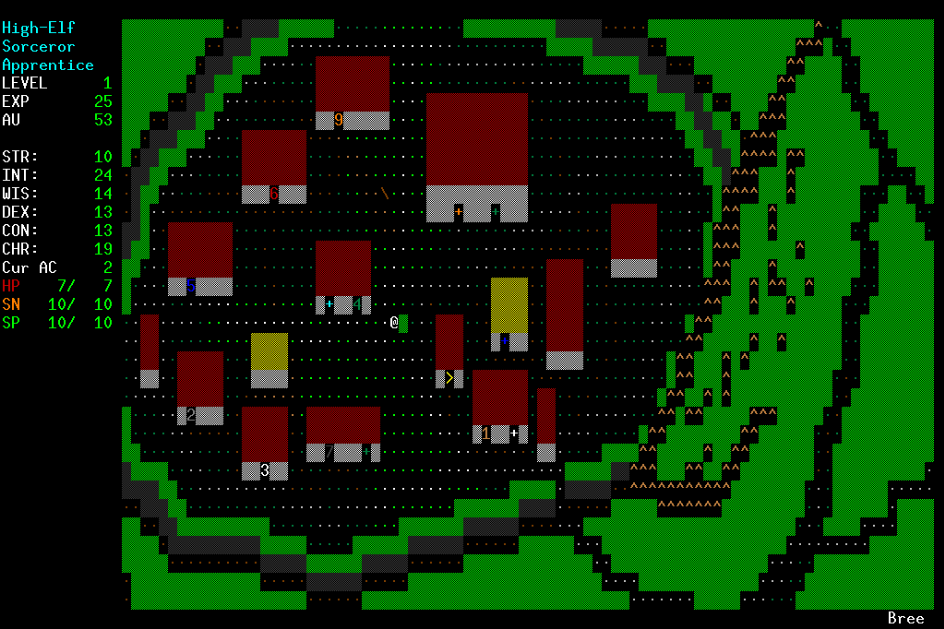
\includegraphics[width=0.9\textwidth]{roguelike.png}
                \end{center}
            \end{column}
        \end{columns}
    \end{frame}

    \begin{frame}
        \frametitle{Что сейчас делать}
        \begin{itemize}
            \item Создать проект, расшарить его мне в личку
            \item Написать комментарием на диаграмме состав команды
            \item Использовать каналы команд для общения внутри команды (опционально)
            \item За 10 минут до конца пары собираемся в общем чате и представляем результаты
        \end{itemize}
    \end{frame}

    \begin{frame}
        \frametitle{Рекомендации}
        \begin{itemize}
            \item Как обычно, проектируйте от общего к частному, не закапывайтесь в детали
            \item Рассмотрите не только структуру данных, но и потоки управления
            \begin{itemize}
                \item Как выполняется пользовательский ввод?
                \item Как передаются ходы, когда вызывается ИИ мобов?
                \item Как инициализируется система?
            \end{itemize}
            \item Помните про модульность и высокоуровневую структуру!
            \begin{itemize}
                \item Разделение на уровни, выбор архитектурного стиля (для каждого уровня отдельно или всей системы целиком)
            \end{itemize}
        \end{itemize}
    \end{frame}

\end{document}